\documentclass[../Main/main.tex]{subfiles}
\begin{document}
	\chapter{Convergence of the MPFA-L Method}
	\label{chap:convergence spatial mpfa}
	\graphicspath{{../Equivalence between MPFA-L and FEM/figs/}}
	In this chapter we show equivalence between a modified MPFA-L method and a modified Lagrange finite element method, for linear time dependent problems discretized in time with backward Euler  \eqref{eq:semidiscrete heat}.
	 That is, we prove equivalence between the two discretizations  of the equation: Let $x\in \Omega \subset \mathbb{R}^2$, find $u(x)$ such that
	\begin{equation}\label{eq:stationary_heat}
	\left \{
	\begin{aligned}[c]
		u - \nabla \cdot\bm{K} \nabla u &= f, \\
		u &= 0, \\
		-\pmb{K}\nabla u &= g_N,
	\end{aligned}
	\ \ \
	\begin{aligned}[c]
		\text{ in }& \Omega \\
		\text{ on }& \partial \Gamma_D \\
		\text{ on }& \partial \Gamma_N ,
	\end{aligned}
	\right.
	\end{equation}
	where $\bm{K}$ is homogeneous, in addition to being symmetric positive definite.
	Once equivalence is obtained, we prove convergence for the finite element method using techniques from section \ref{sec:convergence}. 
	\par
	After reading this chapter, the reader should be convinced that the finite element method covered in section \ref{sec:fem} is almost the same as the L-method. Moreover, that the L-method can be used as a locally mass conservative flux recovery algorithm on the modified finite element solution. See section \ref{sec:elliptic_numerical} for a comparison of the MPFA-L method and normal linear Lagrange finite element method.
	\par
	We saw in the section about the MPFA-L method that the interaction regions (L-triangles) may form a triangulation of our domain.
	With this observation in mind, modifications are made to both methods so that we obtain equivalence. This entire chapter is adapted from (Cao, Y., Helmig, R. and Wohlmuth, B.I. (2009),\cite{https://doi.org/10.1002/num.20525}), where, convergence is proved for the Poisson equation, i.e., without the first term $u$.
	\section{Modified MPFA-L Method}
	\label{sec:modified_mpfa-l}
	First of all, we assume that we have a uniform parallelogram grid, as in \ref{fig:paralellogram-L}. 
	%\begin{figure}[H]\label{fig:paralellogram mesh}
	%	\centering
	%	%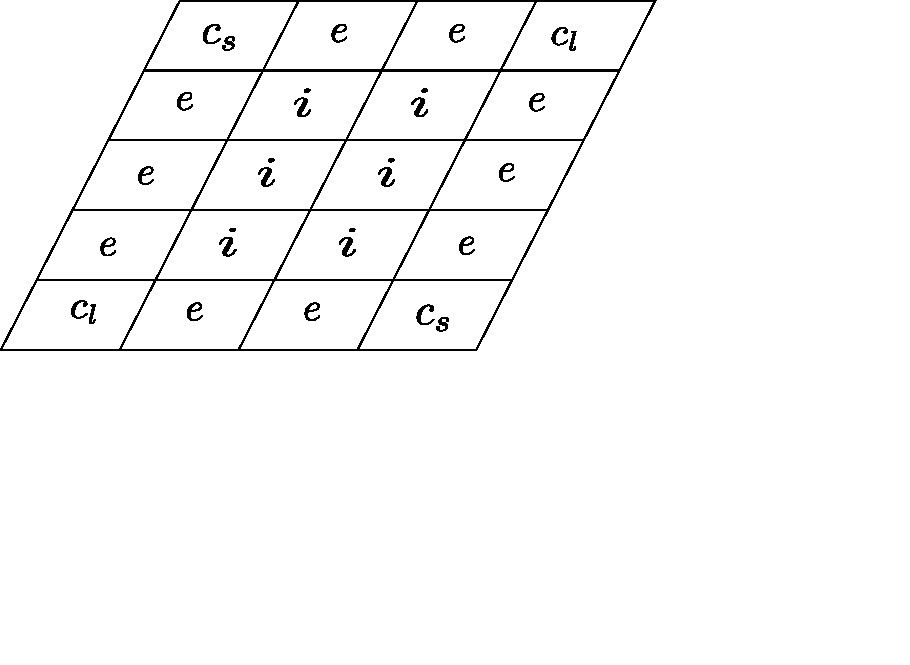
\includegraphics[width=1\textwidth]{paralellogram_mesh.pdf}
	%\end{figure}
	As we saw in the previous chapter, one gets with the finite volume method the following relation for all control volumes $\Omega_i$:
	\begin{equation}
		\int_{\Omega_i} u \ dx - \int_{\partial \Omega_i}\bm{K}\nabla u \cdot \hat{\pmb{n}}\ dx = \int_{\Omega_i} f \ dx.
	\end{equation}
	The MPFA-L method deals with the second term, approximating the constitutive law. The other two terms are common to all control volume methods solving time dependent problems or \eqref{eq:stationary_heat}.
	\par
	On the interior control volumes, we use the original MPFA-L method already covered. On the Neumann boundaries we need a modification. This is to be expected, as control volume methods handle flux at the boundary in a very simple way; specifying it the same way we deal with with the source term, adding it to the load vector. In finite element methods however, we have degrees of freedom on the boundary, one dimensional elements. We will also make a special treatment of the Dirichlet boundary, in a way that is equivalent to the finite element method. In \cite{https://doi.org/10.1002/num.20525} they claim that this is a very natural way of dealing with the Dirichlet boundary conditions, and a good practical alternative to other ways of enforcing Dirichlet boundaries in the MPFA-L method.
	\par
	\begin{figure}
		\centering
		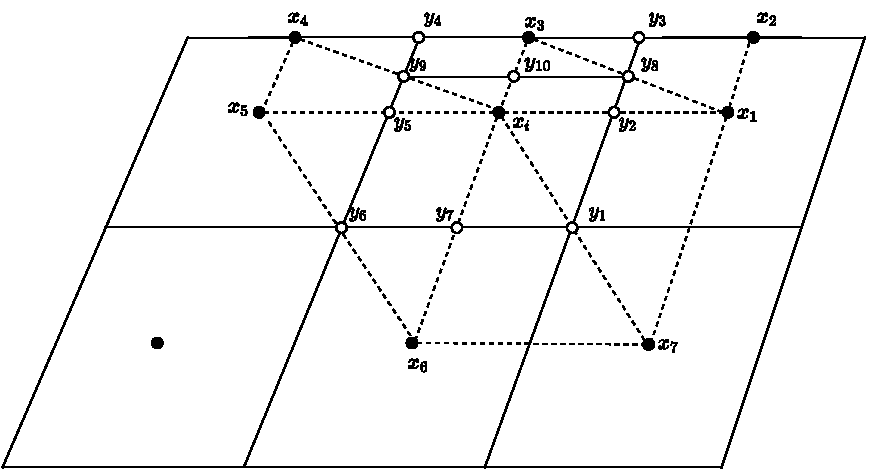
\includegraphics{modified_L_scheme.pdf}
		\caption{Control volumes in solid lines and interaction regions in dashed lines at the boundary.}
		\label{fig:volemes along boundary}
	\end{figure}
	\begin{figure}
		\centering
		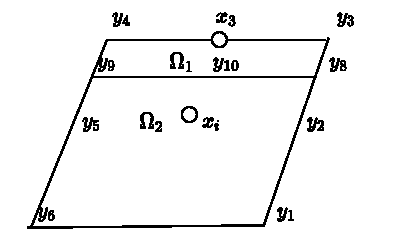
\includegraphics{volumepartition.pdf}
		\caption{Control volume along top boundary.}
		\label{fig:volumepartition}
	\end{figure}
	Consider the control volume $y_1 y_6 y_4 y_3$. 
	For the \textbf{Neumann} boundary conditions, we split the control volume into two, $y_1 y_6 y_9 y_8$ as $\Omega_2$ and $y_8 y_9 y_4 y_3$ as  $\Omega_1$, see figure \ref{fig:volumepartition} or \ref{fig:volemes along boundary}. We therefore get one  equation each for $u_3$ and $u_i$ as the potential at $x_3$ and $x_i$. For the fluxes on $\Omega_2$ we have six interaction triangles and a normal seven point stencil. For the $\Omega_1$ we compute the flux through $\overline{y_3 y_8}$ using $\triangle x_1 x_3 x_2$, the flux through $\overline{y_8 y_{10}}$ using $\triangle x_1 x_i x_3$, for $\overline{y_{10}y_9}$ and $\overline{y_9 y_4}$ the L triangle  $\triangle x_i x_4 x_3$ is used. Finally the Neumann boundary condition is used at the the edge $\overline{y_4 x_3}$ and $\overline{x_3 y_3}$. We are not able to eliminate the unknown value at $x_3$ and it remains a degree of freedom, which makes sense if we want equivalence with finite element method.
	\par
	In the case of \textbf{Dirichlet} boundary conditions, we compute the fluxes into $y_1 y_6 y_4 y_3$ using seven L-triangles, as can be seen in figure \ref{fig:volemes along boundary}. The flux over the edge $\overline{y_3 y_1}$ are computed as the sum of the flux over $\overline{y_3 y_8}$, $\overline{y_8 y_2}$ and $\overline{y_2 y_1}$ using the L-triangles $\triangle x_1 x_3 x_2$, $\triangle x_1 x_i x_3$ and $\triangle x_1 x_7 x_i$ respectively. Similarly for the edge $\overline{y_6 y_4}$. For $\overline{y_1 y_6}$ we only use the two big L-triangles at the bottom, $\triangle x_i x_7 x_6$ and $\triangle x_i x_6 x_5$. 
	\par 
	The flux over $\overline{y_4 y_3}$, at the boundary, we compute by balancing with the other fluxes out of the small control volume $\Omega_1$, see figure \ref{fig:boundary volume Dirichlet}. Let $	\tilde{q}_{\overline{y_i y_j}}$ be the flux through edge $\overline{y_i y_j}$, out of the volume $\Omega_1$. Then we get the expression for the flux through the Dirichlet boundary:
	\begin{equation}\label{eq:K2}
		\tilde{q}_{\overline{y_3 y_4}} =-( \tilde{q}_{\overline{y_3 y_8}} + \tilde{q}_{\overline{y_{10} y_{8}}}+\tilde{q}_{\overline{y_{9}y_{10}}}+\tilde{q}_{\overline{y_4 y_9}}) + \int_{\Omega_1} f \ dx.
	\end{equation}
	The fluxes on the right hand side of \eqref{eq:K2} are computed as for the Neumann case.
	\par
	On the \textbf{corners}, special treatment is needed. Our modified MPFA-L method is modified to become equivalent to the  finite element method here. This is done by splitting the corner control volume into four smaller cells, where mass conservation does not necessarily hold, see \cite{https://doi.org/10.1002/num.20525} for details.
	\begin{figure}
		\centering
		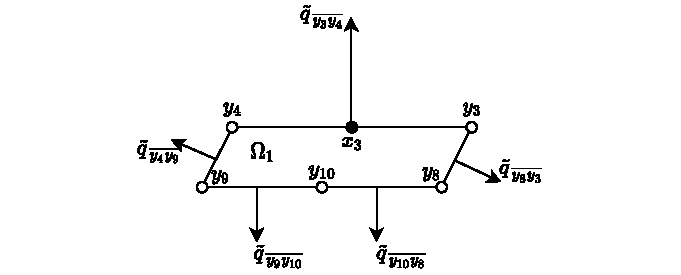
\includegraphics{boundary volume Dirichlet.pdf}
		\caption{The fluxes on the Dirichlet boundary. }
		\label{fig:boundary volume Dirichlet}
	\end{figure}
	\section{Modified Finite Element Method}
	In this section we introduce a finite element method for solving \eqref{eq:stationary_heat}. By theorem \ref{th:L_triangulation} the L-triangles form a triangulation $\left \{ \tau_h \right \}$, we will use linear Lagrange elements on this triangulation. The only modifications we need to make are to the mass matrix and the load vector, we let the stiffness matrix stay the same as before. That is, we do not touch the discretization of the constitutive law. We do want however, to define an interpolation operator such that the inner products that make up the mass matrix and load vector, become mass conservative in each control volume. 
	\par
	We need some notation so that we can distinguish between the cell centers in the interior, at cell centers along the boundary and the nodes at the boundary. In addition, corner cells need special treatment. 
	Let $\mathcal{N}_h^*$ be a set of indices corresponding to all interior nodes of $\left \{ \tau_h \right \}$, which are also the cell centers of the control volume mesh. This index set contains two disjoint sets $\mathcal{N}_h^* = \mathcal{N}_h^b \bigcup \mathcal{N}_h^i$, where superscript $i$ denotes the cell centers of the interior cells and $b$ the boundary cells. The index set $\mathcal{N}^b_h$ are further subdivided as we see in figure \ref{fig:mesWithNodes}. The nodes at the boundary is indexed by the set $\mathcal{N}_h^N \bigcup \mathcal{N}_h^D$, where $N$ and $D$ represent Neumann and Dirichlet boundary nodes, these are further subdivided as illustrated in figure \ref{fig:mesWithNodes}.
	\begin{figure}[H]
		\centering
		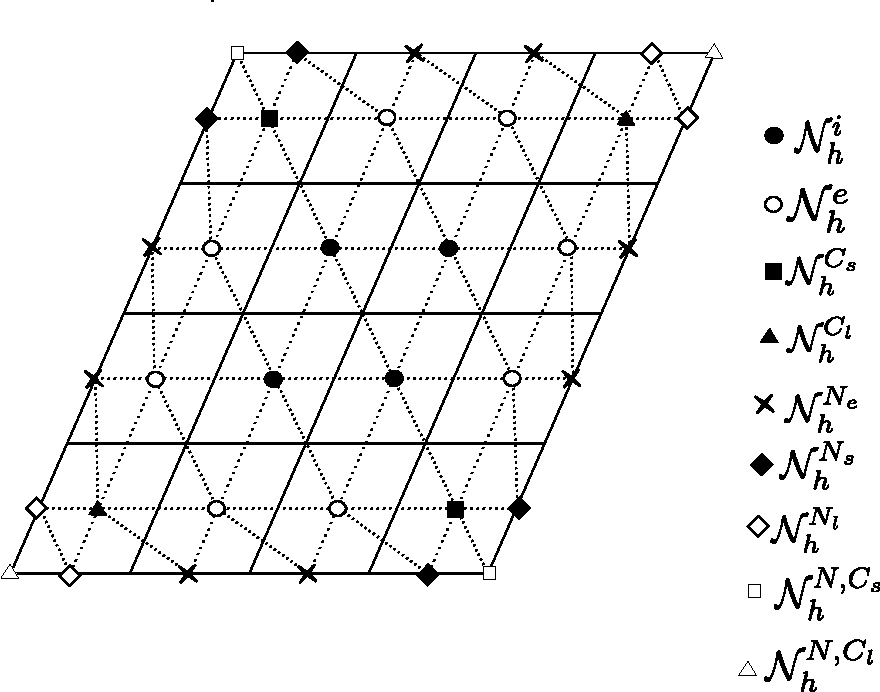
\includegraphics{meshWithNodes.pdf}

		\caption{A paralellogram mesh with finite element triangles in dotted lines and control volumes in solid lines. In this case we have a pure Neumann problem.}
		\label{fig:mesWithNodes}
	\end{figure}
	\par 
	As before we denote by $V_h$ the linear ansatz space as in definition \ref{def:linear ansatz}:
	\begin{equation*}
	V_h = \left \{ u_h \in C(\overline{\Omega}) : u_{h|K} \in \mathcal{P}_1(K) \ \forall K \in \tau_h, u|_{\Gamma_D} = 0  \right \}
	\end{equation*}
	 similarly $\phi_i$ is the standard nodal basis function, where $i \in \mathcal{N}_h \setminus \mathcal{N}_h^D$.
	In addition to our global interpolation operator, definition \ref{def:global_interpolator}, we define an operator that maps functions $v_h \in V_h$ to functions that are piecewise constant on the control volumes. This piecewise function are equal to $v_h$ at the nodes of the triangulation. This is an example of \emph{mass lumping}, see \cite{baranger1996connection} for more examples.
	\begin{definition}[Piecewise global interpolator] \label{def:piecewise_interpolator}
		Let $\hat{I}_h$ be an operator that maps from the test space to functions that are piecewise constant on control volumes.
		\begin{equation*}
			\hat{I}_h:V_h\rightarrow L^2(\Omega)
		\end{equation*}
		And
		\begin{equation*}
			\hat{I}_h v_h = \sum_{i\in \mathcal{N}_h\setminus\mathcal{N}_h^d}v_h(x_i)\hat{I}_h\phi_i(x)
		\end{equation*}
		Where
		\begin{equation}\label{eq:basisfunctionLumped}
			\hat{I}_h\phi_i(x)=\left\{\begin{matrix}
				1 & \text{if } x\in D_i\\ 
				0 & \text{otherwise}
			\end{matrix}\right.
		\end{equation}
		In interior cells, $i\in \mathcal{N}_h^i$, we have $D_i = \Omega_i$, i.e., the support of \eqref{eq:basisfunctionLumped} is the control volume corresponding to $\phi_i$. If we are close or on the boundary the situation is more complicated: 
		\begin{itemize}
			\item $i \in \mathcal{N}_h^e$: In this case the function vanishes for the quarter of the paralellogram closest to the boundary,i.e., $D_i = \Omega_2$ from figure \ref{fig:volumepartition}
			\item $i \in \mathcal{N}_h^{N,e}$ In this case of the neumann boundary node $	\hat{I}_h\phi_i(x)$ vanishes outside the quarter of the control volume closest to the edge,i.e., $D_i = \Omega_1$ in figure \ref{fig:volumepartition}
			\item On the corners there are special definitions, see (Cao Wolmuth \cite{https://doi.org/10.1002/num.20525},2009)
		\end{itemize} 
	\end{definition}
	Let $\hat{I}_{\Gamma_N} = \hat{I}_{h}|_{\Gamma_N}$ be the trace of the piecewise interpolation operator on the neumann boundary.
	The finite element method we end up with reads as follows: Find $u_h\in V_h$ such that
	\begin{equation} \label{eq:modified_fem}
			\left \langle \hat{I}_h u_h,\hat{I}_h v_h \right \rangle_{0,\Omega} +   \left \langle\bm{K} \nabla u_h,\nabla v_h \right \rangle_{0,\Omega} = \left \langle f,\hat{I}_h v_h \right \rangle_{0,\Omega} + \left \langle g,\hat{I}_{\Gamma_N} v_h \right \rangle_{0,\Gamma_N},
	\end{equation}
	for all $v_h\in V_h$. 
	The key takeaway here is the local support of the inner products, this will make the mass matrix diagonal.   
	\par
		\begin{figure}[H]
		\centering
		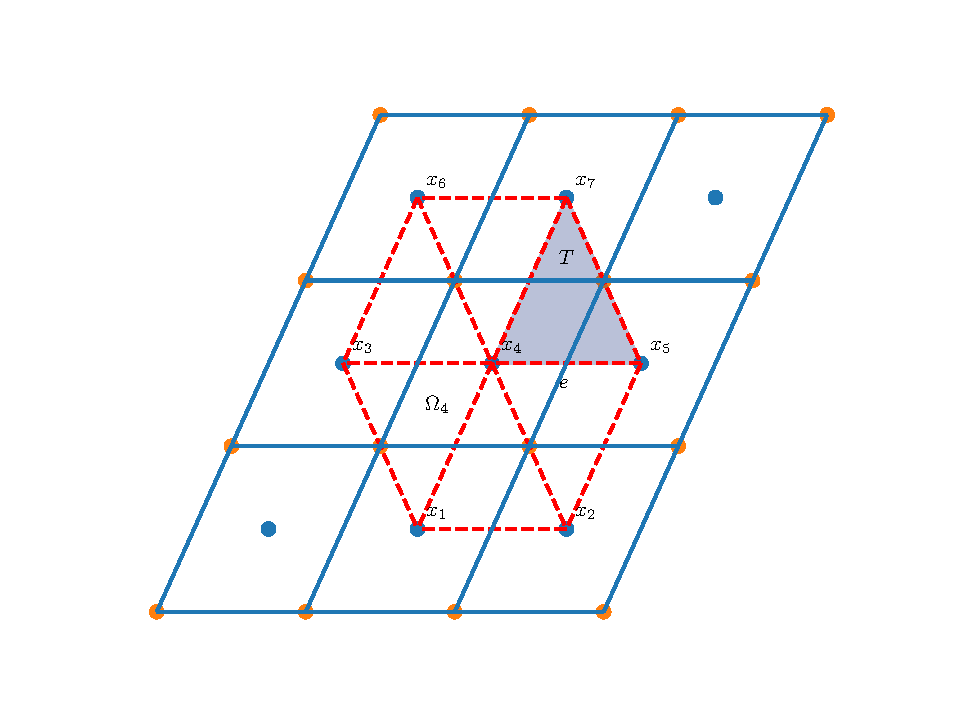
\includegraphics[width=1\textwidth]{Control volume.pdf}
		\caption{The support of $\phi_4$, the coloured area corresponds to one triangle (element) in the support of $\phi_4$. }
		\label{fig:control volume}
	\end{figure}
	\begin{figure}[H]
		\centering
		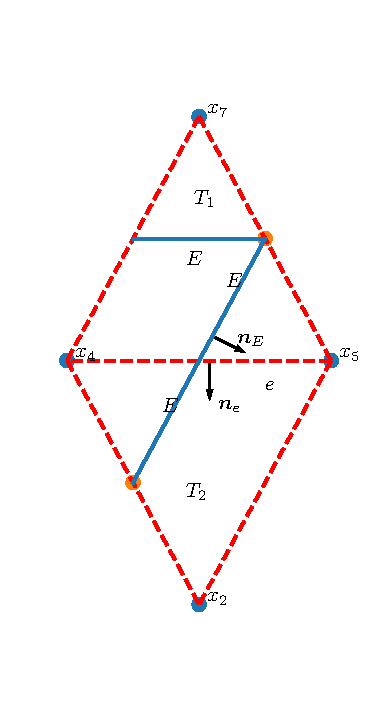
\includegraphics{two triangles.pdf}
		\caption{Notation in the proof}
		\label{fig:two triangles}
	\end{figure}
	Now we can state the equivalence theorem:
	\begin{theorem}
		The modified finite element method \eqref{eq:modified_fem} and the modified MPFA-L method are equivalent on uniform parallelogram grid for the time discretized heat equation,i.e., \eqref{eq:stationary_heat}, on homogeneous media. 
	\end{theorem}

	\begin{proof}
		We do the proof in four steps:
		\begin{enumerate}
			\item First, we show the equivalence for the interior, so
			let $\Omega_i$ be an interior control volume and $\phi_i$ be the corresponding basis function evaluating to one at the centre of $\Omega_i$, where $i \in \mathcal{N}_h^i$.
			We test \eqref{eq:modified_fem} with $v_h=\phi_i$:
			\begin{equation}\label{eq:modified fem interior}
				\left \langle \hat{I}_h u_h,\hat{I}_h \phi_i \right \rangle_{0,\Omega} +   \left \langle\bm{K} \nabla u_h,\nabla \phi_i \right \rangle_{0,\Omega} = \left \langle f,\hat{I}_h \phi_i \right \rangle_{0,\Omega} .
			\end{equation}
			
			 Let $T \in \tau_h \bigcap \text{supp}(\phi_i)$ be one of the elements in the triangulation that makes up the support of $\phi_i$. $S=T\bigcap \Omega_i$ is a part of the control volume that lies in some element, and $E \subset S\bigcap \partial \Omega_i$ are the half edges of $\Omega_i$. $e$ are the interior edges of $\tau_h$ inside the support of $\phi_i$, see fig \ref{fig:two triangles} and \ref{fig:control volume}. $\bm{n}_e$ is the unit normal on $e$ with fixed and arbitrary orientation, and $\pmb{n}_E$ is the unit normal on $E$ pointing out of $\Omega_i$. Let $T_{e,0}$ and $T_{e,1}$ be the two elements having $e$ as a common edge, with the numbering corresponding to the orientation of $\bm{n}_e$. Since $u_h$ and $\phi_i$ are piecewise linear and $\bm{K}$ is constant on each triangle $T$, we have:
			\begin{equation}\label{eq:big computation}
				\begin{aligned}
					\left \langle\bm{K}\nabla u_h, \nabla \phi_i \right \rangle_0 &= \int_{\text{supp}(\phi_i)} (\bm{K}\nabla u_h)^T\nabla \phi_i \ dx = \sum_{T\in \text{supp}(\phi_i)} \int_T (\bm{K}\nabla u_h)^T\nabla \phi_i \ dx \\
					&= \sum_{T\in \text{supp}(\phi_i)} \left ( \int_{\partial T} (\pmb{K}\nabla u_h)^T\bm{n}\phi_i \ ds-\int_T \nabla \cdot\bm{K} \nabla u_h \phi_i \ dx \right ) \\
					&=\sum_{T\in \text{supp}(\phi_i)}\int_{\partial T} (\bm{K}\nabla u_h)^T\bm{n}\phi_i \ ds \\
					&= \sum_{e\in \text{supp}(\phi_i)} \int_e \left ((\bm{K}\nabla u_h)^T\bm{n}_e|_{T_{e,0}} - (\bm{K}\nabla u_h)^T\bm{n}_e|_{T_{e,1}} \right )\phi_i \ ds\\
					&= \sum_{e\in \text{supp}(\phi_i)}
					\left ((\bm{K}\nabla u_h)^T\bm{n}_e|_{T_{e,0}} - (\bm{K}\nabla u_h)^T\bm{n}_e|_{T_{e,1}} \right ) \frac{|e|}{2}\\
					&=\sum_{S\in \text{supp}(\phi)}\int_{\partial S}  (\bm{K}\nabla u_h)^T\bm{n} \ ds - \sum_{E\in \partial \Omega_i}\int_E (\bm{K}\nabla u_h)^T\bm{n}_E \ ds\\
					&= \sum_{S\in \text{supp}(\phi)}\int_{ S} \nabla \cdot\bm{K}\nabla u_h \ ds - \sum_{E\in \partial \Omega_i}\int_E (\pmb{K}\nabla u_h)^T\bm{n}_E \ ds\\
					&=- \sum_{E\in \partial \Omega_i} (\pmb{K}\nabla u_h)^T\bm{n}_E |E| .
				\end{aligned}
			\end{equation}
			Note that this last sum is a sum of integrals over the half edges of $\Omega_i$. 
			Further, we have that 
			\begin{equation}\label{eq:mass equiv 1}
				\left \langle \hat{I}_h  u_h,\hat{I}_h\phi_i \right \rangle_0 = \int_{\Omega}\hat{I}_h u_h \hat{I}_h \phi_i \ dx =  \int_{\Omega_i}u_h(x_i) \ dx
			\end{equation}
			and
			\begin{equation}\label{eq:load equiv 1}
				\left \langle f,\hat{I}_h \phi_i \right \rangle_0 = \int_{\Omega_i}f \ dx.
			\end{equation}
			Combining equation \eqref{eq:big computation}, \eqref{eq:mass equiv 1} and \eqref{eq:load equiv 1} we get that \eqref{eq:modified fem interior} is equivalent to:
			\begin{equation}
				\int_{\Omega_i}u_h(x_i) \ dx - \sum_{E\in \partial \Omega_i} (\pmb{K}\nabla u_h)^T\bm{n}_E |E| = \int_{\Omega_i}f \ dx.
			\end{equation}
			We know from theorem \ref{lemma:L_potential} that the flux over each half edge in the L-method is given uniquely by the potential values of the three cell centers in the L-triangle. Since the L-triangles and the elements are the same, $\nabla u_h$ corresponds to the gradient used in the L-method, see equation \eqref{eq:L flux simplified}. Hence, if $\hat{u}_h$ is the solution to \eqref{eq:stationary_heat} with the original L-method in the interior, then $\hat{u}_h(x_i)=u_h(x_i)$ for $x_i\in \mathcal{N}^i_h$. 
			\item For a control volume bordering the \textbf{Neumann} boundary, first let $i\in \mathcal{N}_h^e$, we have:
			\begin{equation}\label{eq:case2}
				\left \langle \hat{I}_h u_h,\hat{I}_h \phi_i \right \rangle_{0,\Omega} +   \left \langle\bm{K} \nabla u_h,\nabla \phi_i \right \rangle_{0,\Omega} = \left \langle f,\hat{I}_h \phi_i \right \rangle_{0,\Omega}.
			\end{equation}
			With similar computations and reasoning as for \eqref{eq:big computation} we get:
			\begin{equation}
					\left \langle\bm{K} \nabla u_h,\nabla \phi_i \right \rangle_{0,\Omega}= 
					- \sum_{E\in \partial \Omega_{i,2}} (\pmb{K}\nabla u_h)^T\bm{n}_E |E|, 
			\end{equation}
			where $\Omega_{i,2}$ is as $\Omega_2$ in figure \ref{fig:volumepartition}. As $\hat{I}_h$ is carefully defined close to the Neumann boundary, we get that \eqref{eq:case2} is equivalent to:
			\begin{equation}\label{eq:FVML neumann cell}	\int_{\Omega_{i,2}}u_h(x_i) \ dx - \sum_{E\in \partial \Omega_{i,2}} (\pmb{K}\nabla u_h)^T\bm{n}_E |E| = \int_{\Omega_{i,2}}f(x_i) \ dx.
			\end{equation}
			Next, let $j \in \mathcal{N}_h^{N,e}$,i.e., the index of a node on the boundary. Then we have 
			\begin{equation}\label{eq:case neumann node}
				\left \langle \hat{I}_h u_h,\hat{I}_h \phi_j \right \rangle_{0,\Omega} +   \left \langle\bm{K} \nabla u_h,\nabla \phi_j \right \rangle_{0,\Omega} = \left \langle f,\hat{I}_h \phi_j \right \rangle_{0,\Omega}+ \left \langle g,\hat{I}_{\Gamma_N} \phi_j \right \rangle_{0,\Gamma_N}.
			\end{equation}
			Similarly as in \eqref{eq:big computation} we have
			\begin{equation}\label{eq:case neumann 1}
				\begin{aligned}
						\left \langle\bm{K}\nabla u_h, \nabla \phi_{j} \right \rangle_0 &= \int_{\text{supp}(\phi_{j})} (\bm{K} \nabla u_h)^T\nabla \phi_{j} \ dx = \sum_{T\in \text{supp}(\phi_{j})} \int_T (\bm{K}\nabla u_h)^T\nabla \phi_{j} \ dx \\
					&= \sum_{T\in \text{supp}(\phi_{j})} \left ( \int_{\partial T} (\bm{K}\nabla u_h)^T\bm{n}\phi_{j} \ ds-\int_T \nabla \cdot\bm{K} \nabla u_h \phi_{j} \ dx \right ) \\
					&=\sum_{T\in \text{supp}(\phi_{j})}\int_{\partial T} (\bm{K}\nabla u_h)^T\bm{n}\phi_{j} \ ds.
				\end{aligned}
			\end{equation}
			But because $\phi_{j}\neq 0$ on $\text{supp}(\phi_{j})\bigcap \Gamma_N$, we get
			\begin{equation}\label{eq:case neumann 2}
				\begin{aligned}
					\sum_{T\in \text{supp}(\phi_{j})}\int_{\partial T} (\bm{K}\nabla u_h)^T\bm{n}\phi_{j} \ ds &= \sum_{e\in \text{supp}(\phi_{j})} \int_e \left((\bm{K}\nabla u_h)^T\bm{n}_e|_{T_{e,0}} - (\bm{K}\nabla u_h)^T\bm{n}_e|_{T_{e,1}}\right)\phi_j \ ds\\ &+ \int_{\Gamma_N \bigcap \text{supp}(\phi_{j})}(\bm{K}\nabla u_h)^T\bm{n} \phi_j \ ds\\
					&= \sum_{e\in \text{supp}(\phi_{j})} \left ((\bm{K}\nabla u_h)^T\bm{n}_e|_{T_{e,0}} - (\bm{K}\nabla u_h)^T\bm{n}_e|_{T_{e,1}}\right)\frac{|e|}{2} \ ds\\ &+ (\bm{K}\nabla u_h)^T\bm{n} |E_{\Gamma_N}| \ ds\\
					&= -\sum_{E\in \partial \Omega_{j}\setminus \Gamma_N} (\bm{K}\nabla u_h)^T\bm{n}_E |E|
				\end{aligned}
			\end{equation}
			Combining \eqref{eq:case neumann 1} and \eqref{eq:case neumann 2} and using the definition of $\hat{I}_h$, definition \ref{def:global_interpolator}, we get that \eqref{eq:case neumann node} is equivalent to:
			\begin{equation}\label{eq:FVML neumann node}
				\int_{\Omega_{j,1}}u_h(x_i) \ dx - \sum_{E\in \partial \Omega_{j,1}} (\bm{K}\nabla u_h)^T\bm{n}_E |E| = \int_{\Omega_{j,1}}f(x_i) \ dx.
			\end{equation}
			Where $\Omega_{j,1}$ is as $\Omega_1$ in figure \ref{fig:volumepartition}. Now, \eqref{eq:FVML neumann cell} and \eqref{eq:FVML neumann node} are exactly the L-method for the Neumann boundary, as described earlier, see figure \ref{fig:volemes along boundary}.  
			\item For a control volume near the \textbf{Dirichlet} boundary, let first $i\in \mathcal{N}_h^e$,i.e., the cell center. Then, our modified finite element method
			\begin{equation}
				\left \langle \hat{I}_h u_h,\hat{I}_h \phi_j \right \rangle_{0,\Omega} +   \left \langle\bm{K} \nabla u_h,\nabla \phi_j \right \rangle_{0,\Omega} = \left \langle f,\hat{I}_h \phi_j \right \rangle_{0,\Omega}
			\end{equation}   
			is equivalent to 
			\begin{equation} 
				\int_{\Omega_{i,2}} u_h (x_i) \ dx- \sum_{E\in \partial \Omega_{i,2}} (\pmb{K}\nabla u_h)^T\bm{n}_E |E| = \int_{\Omega_{i,2}} f \ dx,
			\end{equation} 
			with the same reasoning as in \eqref{eq:big computation}, \eqref{eq:mass equiv 1} and \eqref{eq:load equiv 1}. As $\Omega_i = \Omega_{i,1}\bigcup \Omega_{i,2}$ and $\Omega_{i,1}\bigcap \Omega_{i,2}= \emptyset$, see figure \ref{fig:volumepartition}, we have:
			\begin{equation}
				-\sum_{E\in \Omega_i \setminus \Gamma_D}(\pmb{K}\nabla u_h)^T\bm{n}_E |E| + \sum_{E\in \Omega_{i,1} \setminus \Gamma_D}(\pmb{K}\nabla u_h)^T\bm{n}_E |E| + \int_{\Omega_{i,1}} f \ dx = \int_{\Omega_i} f \ dx.
			\end{equation}
			We recognize the second and third terms in the above equation as the flux across the Dirchlet boundary in the modified L method, see \eqref{eq:K2}.
			\item See \cite{https://doi.org/10.1002/num.20525} for equivalence on the corner cells.
		\end{enumerate}
	\end{proof}
	\section{Convergence Rate Estimates}
	Our modified finite element method only approximates the bi-linear and linear form, and we need to take this into account when proving a convergence rate estimate. The following lemma is an extension of Cèa's lemma \ref{lemma:cea}, it is useful for estimating the error when our bi-linear and linear form is not exact.
	\begin{lemma}[First Lemma of Strang, page 155 \cite{Knabner}]\label{lemma:strang}
		Suppose there exists some $\alpha>0$ such that for all $h>0$ and $v_h\in V_h$
		\begin{equation*}
			\alpha \left \| v_h \right \|^2_1 \leq a_h(v_h,v_h) 
		\end{equation*}
		and let $a$ be continuous in $V\times V$. Then there exist some constant $C$ independent of $V_h$ such that
		\begin{equation}\label{eq:strang_ineq}
			\begin{aligned}
				\left \| u-u_h \right \|_1 \leq C&\left \{ \inf_{v_h \in V_h}\left \{ \left \| u-v_h \right \|_1 +  \sup_{w_h\in V_h}\frac{|a(v_h,w_h)-a_h(v_h,w_h)|}{\left \| w_h \right  \|_1}\right \}   \right. \\ 
				&+\left. \sup_{w_h\in V_h}\frac{|l(w_h)-l_h(w_h)|}{\left \| w_h \right \|_1}    \right \}			
			\end{aligned}
		\end{equation}
	\end{lemma}
	From \eqref{eq:modified_fem} we see that we have a bi-linear form 
	\begin{equation}
		a_h(u_h,v_h) = \left \langle \hat{I}_h u_h, \hat{I}_h v_h \right \rangle_{0,\Omega} +  \left \langle\bm{K} \nabla u_h, \nabla v_h \right \rangle_{0,\Omega}.
	\end{equation}
	And the linear form:
	\begin{equation}
		b_h(v_h)= \left \langle F,\hat{I}_h v_h \right \rangle_{0,\Omega} + \left \langle g,\hat{I}_{\Gamma_N} v_h \right \rangle_{0.\Gamma_N}.
	\end{equation}
	To apply the first Lemma of Strang \ref{lemma:strang}, we first show that $a_h(\cdot,\cdot)$ is coercive. We write out the Sobolev norm
	\begin{equation}
			\left \| u_h \right \|_1^2  = \left \langle \nabla u_h,\nabla u_h \right \rangle_0 + \left \| u_h \right \|_0^2. 
		\end{equation}
		Using the Poincaré inequality on the second term:
		\begin{equation}
		\begin{aligned} 
		\left \| u_h \right \|_1^2	&\leq \left \langle \nabla u_h,\nabla u_h \right \rangle_0 + C_{\Omega} \left \langle \nabla u_h, \nabla u_h \right \rangle_0 \\
			&\leq \left(\frac{1+C_{\Omega}}{\tau \left \|\bm{K}\right \|} \right) \tau \left  \langle  \bm{K} \nabla  u_h, \nabla u_h \right \rangle_0  \\
			&\leq \left(\frac{1+C_{\Omega}}{\tau \left \|\bm{K}\right \|} \right) \left(\tau \left  \langle  \bm{K} \nabla  u_h, \nabla u_h \right \rangle_0 + \left \langle \hat{I}_h u_h,\hat{I}_h u_h \right \rangle_0\right)\\
			&= \frac{1}{\alpha} a_h(u_h,u_h), 
		\end{aligned}
	\end{equation} 
	we obtain coercivity with $\alpha = \tau \left \|\bm{K}\right \|/(1+C_{\Omega})$, where $C_{\Omega}$ is some constant depending on the domain and the boundary conditions.\par
	Another important piece that must be in place for a convergence proof is the piecewise interpolation error:
	\begin{lemma}\label{lemma:int_error}
		For the previously defined piecewise global interpolator $\hat{I}_h$, definition \ref{def:piecewise_interpolator}, we have the estimate:
		\begin{equation}
			\left \| \hat{I}_h u_h - u_h \right \|_{0,\Omega} \leq C h | u_h |_{1,\Omega} \ \forall u_h \in V_h,
		\end{equation}
		for some constant $C$ independent of the mesh diameter.
	\end{lemma}
	\begin{proof}
		\begin{equation}
			\begin{aligned}
				\left \| \hat{I}_h u_h - u_h \right \|^2_0 &= \sum_{i\in \mathcal{N}_h^*} \left \|\hat{I}_h u_h - u_h\right \|^2_{0,\Omega_i} \\
					&=\sum_{i\in \mathcal{N}_h^*} \int_{\Omega_i}\left(u_h(x_i)-u_h(x)  \right)^2 \ dx\\
					&=\sum_{i\in \mathcal{N}_h^*} \int_{\Omega_i}h^2\left(\frac{u_h(x_i)-u_h(x)}{h}  \right)^2 \ dx\\
					&\leq \sum_{i\in \mathcal{N}_h^*} \int_{\Omega_i} h (\nabla u_h)^T \nabla u_h \ dx\\
					&=Ch|\nabla u_h|_1^2
			\end{aligned}
		\end{equation}
	\end{proof}
	We are now ready to state the $H^1$ error estimate for the modified finite element method and thus the MPFA-L method.
	\begin{theorem}\label{th:convergence of elliptic}
		Let $u$ solve \eqref{eq:stationary_heat} and $u_h$ be the solution resulting from MPFA-L , then there exists a positive constant $C$ independent of the mesh diameter, $h$, such that
		\begin{equation}\
			\left \|u - u_h \right \|_1 \leq C h (\left \| u \right \|_2 + \left \| f \right \|_0 + \left \| g \right \|_{\frac{1}{2},\Gamma_N}).
		\end{equation}
	\end{theorem}
	\begin{proof}
		The hypothesis in Strang's lemma \ref{lemma:strang} on continuity and coercivity are fulfilled. Let $C$ be a generic positive constant.
		We start by controlling the second term on the right hand side in \eqref{eq:strang_ineq}, the truncation error in the bi-linear form:
		\begin{equation}
			\begin{gathered}
				\sup_{w_h\in V_h} \frac{|a(v_h,w_h)-a_h(v_h,w_h)|}{\left \|w_h \right \|_1} \\
				=\sup_{w_h\in V_h} \frac{|\left \langle v_h,w_h\right \rangle + \tau \left \langle\bm{K} \nabla v_h,\nabla w_h \right \rangle - \left \langle \hat{I}_h v_h, \hat{I}_h w_h \right \rangle - \tau \left \langle\bm{K} \nabla v_h, \nabla w_h \right \rangle|}{\left \| w_h \right \|_1} \\
				=\sup_{w_h\in V_h} \frac{|\left \langle v_h,w_h\right \rangle - \left \langle \hat{I}_h v_h, w_h \right \rangle + \left \langle \hat{I}_h v_h, w_h \right \rangle - \left \langle \hat{I}_h v_h, \hat{I}_h w_h \right \rangle|}{\left \| w_h \right \|_1}\\
				= \sup_{w_h\in V_h}\frac{|\left \langle \hat{I}_h v_h - v_h,w_h \right \rangle + \left \langle \hat{I}_h v_h, \hat{I}_h w_h - w_h \right \rangle |}{\left \| w_h \right \|_1}. \\
			\end{gathered}
		\end{equation}
		We see from the above computations, that the truncation error in the bi-linear form, only has a contribution from the \emph{mass lumping}.
		By Cauchy Schwarz inequality and lemma \ref{lemma:int_error} we get:
		\begin{equation}
			\begin{gathered}
				\leq \sup_{w_h\in V_h}\frac{Ch| v_h|_1\left \| w_h \right \|_0  + \left \|\hat{I}_h v_h\right \|_0 Ch|w_h|_1}{\left \| w_h \right \|_1}\\
				\leq 				 \sup_{w_h\in V_h}\frac{Ch| v_h|_1\left \| w_h \right \|_0  + \left \|\hat{I}_h v_h\right \|_0 Ch|w_h|_1}{\left \| w_h \right \|_1} + \frac{Ch\left \| v_h \right \|_0 \left \| w_h \right \|_0 + \left \|\hat{I}_h v_h\right \|_0 Ch\left \| w_h \right \|_0}{\left \| w_h \right \|_1}\\
				\leq Ch \left (\left \| v_h \right \|_0 + \left \| \hat{I}_h v_h \right \|_0 \right ).
			\end{gathered}
		\end{equation}
		The third term in \eqref{eq:strang_ineq}, the linear form, can be controlled similarly:
		\begin{equation}\label{eq:334}
			\begin{aligned}
				\sup_{w_h \in V_h} \frac{l(w_h)-l_h(w_h)}{\left \| w_h \right \|_1} &= \sup_{w_h \in V_h} \frac{\left \langle f,w_h-\hat{I}_h w_h \right \rangle_{0,\Omega} + \left \langle g,w_h-\hat{I}_{\Gamma_N} w_h \right \rangle_{0,\Gamma_N}}{\left \| w_h \right \|_1}\\
				&\leq \sup_{w_h \in V_h} \frac{\left \|f\right \|_0 Ch\left \|w_h \right \|_1 + \left \|g\right \|_{\frac{1}{2},\Gamma_N}\left \|w_h-\hat{I}_{\Gamma_N} w_h\right \|_{-\frac{1}{2},\Gamma_N}}{\left \| w_h \right \|_1}.
			\end{aligned}
		\end{equation}
		Now, we want to bound $\left \|w-\hat{I}_{\Gamma_N} w_h\right \|_{-\frac{1}{2},\Gamma_N}$ by $\left \| w_h \right \|_1$. Let $v_h$ be a piecewise constant function on the boundary in each Neumann boundary triangle. Then we have:
		\begin{equation}
			\begin{aligned}
				\left \|w_h-\hat{I}_{\Gamma_N} w_h\right \|_{-\frac{1}{2},\Gamma_N} &= \sup_{0 \neq v \in H^{\frac{1}{2}}(\Omega)}\frac{\left \langle w_h-\hat{I}_{\Gamma_N} w_h,v\right \rangle_{\Gamma_N}}{\left \| v \right \|_{\frac{1}{2},\Gamma_N}}\\
				&=\sup_{0 \neq v \in H^{\frac{1}{2}}(\Omega)}\frac{\left \langle w_h-\hat{I}_{\Gamma_N} w_h,v-v_h\right \rangle_{\Gamma_N}}{\left \| v\right \|_{\frac{1}{2},\Gamma_N}},
			\end{aligned}
		\end{equation}
		as $\int_{\Gamma_N} (w_h-\hat{I}_{\Gamma_N} w_h) \ dx = 0$. Now, we can use Cauchy Schwarz inequality:
		\begin{equation}\label{eq:neumann CS estimate}
			\left \|w_h-\hat{I}_{\Gamma_N} w_h\right \|_{-\frac{1}{2},\Gamma_N} \leq \sup_{0 \neq v \in H^{\frac{1}{2}}(\Omega)}\frac{\left \| w_h-\hat{I}_{\Gamma_N} w_h\right \|_{0,\Gamma_N}\left \| v-v_h\right \|_{0,\Gamma_N}}{\left \| v\right \|_{\frac{1}{2},\Gamma_N}}.
		\end{equation}
		By the inequality
		\begin{equation}\label{eq:difficult inequality}
			\left \| v-v_h\right \|_{0,\Gamma_N} \leq C h^{\frac{1}{2}} \left \| v \right \|_{\frac{1}{2}, \Gamma_N},
		\end{equation}
		we can bound the right hand side of  \eqref{eq:neumann CS estimate}: 
		\begin{equation}
				\left \|w_h-\hat{I}_{\Gamma_N} w_h\right \|_{-\frac{1}{2},\Gamma_N} \leq Ch^{\frac{1}{2}} \left \| w_h-\hat{I}_{\Gamma_N} w_h \right \|_{0,\Gamma_N}.
		\end{equation}
		Using \eqref{eq:difficult inequality} again, we get
		\begin{equation}
				\left \|w_h-\hat{I}_{\Gamma_N} w_h\right \|_{-\frac{1}{2},\Gamma_N} \leq Ch \left \|w_h\right \|_{\frac{1}{2},\Gamma_N} \leq Ch\left \| w_h \right \|_1.
		\end{equation}
		Where the last inequality is due to the definition of the $H^{\frac{1}{2}}$ norm. Inserting this into \eqref{eq:334}, gives us a bound on the truncation error of our linear form:
		\begin{equation}
			\sup_{w_h \in V_h} \frac{l(w_h)-l_h(w_h)}{\left \| w_h \right \|_1} \leq Ch(\left \|f \right \|_0 + \left \| g \right \|_{\frac{1}{2},\Gamma_N}).
		\end{equation}
		Hence, from \eqref{eq:strang_ineq}, we have the error estimate:
		\begin{equation}\label{eq:341}
					\left \| u - u_h \right \|_1 \leq \inf_{v_h \in V_h}\left \{ \left \| u - v_h \right \|_1 + Ch \left (\left \| v_h\right \|_0 + \left \| \hat{I}_h v_h \right \|_0 + \left \| f \right \|_0 + \left \| g \right \|_{\frac{1}{2},\Gamma_N}\right ) \right \}.
		\end{equation}
	If we let $v_h = I_h u \in V_h$, in \eqref{eq:341}, where $I_h:C(\Omega) \rightarrow V_h$ is the global interpolation operator, we get the inequality:
	\begin{equation}\label{eq:342}
	\left \| u - u_h \right \|_1 \leq \left \| u - I_h u \right \|_1 + Ch \left (\left \| I_h u\right \|_0 + \left \| \hat{I}_h I_h u \right \|_0 + \left \| f \right \|_0 + \left \| g \right \|_{\frac{1}{2},\Gamma_N} \right ).
	\end{equation}
	As discussed earlier, in section \ref{sec:convergence} about convergence of finite element method, we have the estimate:
	\begin{equation}
 \left \| u - I_h u \right \|_1 \leq C h|u|_2.
	\end{equation}
	If we insert this into \eqref{eq:342}, we get:
	\begin{equation}
	\left \| u - u_h \right \|_1 \leq  Ch \left ( |u|_2 + \left \| I_h u\right \|_0 + \left \| \hat{I}_h I_h u \right \|_0 + \left \| f \right \|_0 + \left \| g \right \|_{\frac{1}{2},\Gamma_N} \right ).
	\end{equation}
	As $I_h u, \hat{I}_h u \rightarrow u$ as $h\rightarrow 0$, we can control the first three terms inside the parenthesis by the $H^2$ norm of $u$, and we get the desired result:
	\begin{equation}
\left \| u - u_h \right \|_1 \leq  Ch \left ( \left \|u\right \|_2 + \left \| f \right \|_0 + \left \| g \right \|_{\frac{1}{2},\Gamma_N} \right ).	\end{equation}
	\end{proof}
	In this chapter we have introduced a way to handle Dirichlet and Neumann boundary conditions for the MPFA-L method, and showed convergence when applied to \eqref{eq:stationary_heat}. The convergence was obtained with showing equivalence to a modified linear Lagrange finite element method.
	\begin{remark}\label{rem:l2_remark}
		In our convergence rate estimate, we showed that $\left \|u-u_h\right \|_1$ decreases proportional to the mesh diameter, $h$. In \cite{https://doi.org/10.1002/num.20525}, the authors show, using the Aubin-Nitsche technique, an estimate where $\left \|u-u_h\right \|_0$ decreases proportional to the square of the mesh diameter. We expect similar results can be shown here, as the equations are similar.
	\end{remark}
\end{document}